\documentclass[preprint,12pt]{elsarticle}
\usepackage{graphicx}
\usepackage{booktabs}
\usepackage{array}
\usepackage{tabularx}
\usepackage{amsmath}
\usepackage{url}
\usepackage{caption}
\usepackage[colorlinks=true,linkcolor=blue,citecolor=blue,urlcolor=blue]{hyperref}
\biboptions{numbers,sort&compress}
\captionsetup{font=footnotesize,labelfont=bf,skip=3pt}
\setlength{\parindent}{1em}
\setlength{\parskip}{0pt}
\setlength{\textfloatsep}{8pt plus 2pt minus 2pt}
\setlength{\floatsep}{7pt plus 2pt minus 2pt}
\setlength{\intextsep}{7pt plus 2pt minus 2pt}
\emergencystretch=3em

\journal{Computational Particle Mechanics}

\begin{document}
\begin{frontmatter}
\title{\texorpdfstring{Bonded-template DEM reveals strength- and topology-dependent fracture-event sequences in packed brittle ceramic pebbles}{Bonded-template DEM reveals strength- and topology-dependent fracture-event sequences in packed brittle ceramic pebbles}}
\author{Anonymous author(s)}










\begin{abstract}

Packed brittle pebbles can lose mechanical integrity through a small number of localized particle fractures before bed-wide fragmentation is visible. Here, we develop a bonded-template discrete-element workflow that inserts 500-subparticle brittle templates into random packed beds with no pre-loading bond loss and records parent-particle fracture events during compression. A nominal 1 mm Li$_4$SiO$_4$ template is calibrated against single-pebble crush-load and split-fragment constraints. Selected 100-parent-particle bed windows retain 493,500 initial internal bonds, measurable load transfer and a connected native force graph before fracture loading. The completed endpoint dataset contains four localized cracking sequences, five zero-loss endpoints, including nominal and 0.25x 200-parent-particle intact scale/strength checks, and an eleven-row material-response table with a six-case strength matrix across two cracking geometries. The early-cracking geometry keeps first localized bond loss at 19 micrometres as strength is reduced from nominal to 0.25x, with endpoint bond loss increasing from 10 to 15 only at 0.25x. The synchronous-cracking geometry shifts first localized bond loss from 39 micrometres at nominal strength to 19 micrometres at 0.50x and 0.25x, again increasing endpoint bond loss to 15 only at 0.25x. These results show that fracture onset in finite packed-particle windows is controlled by the combination of local force-path topology and bonded-particle strength. The workflow converts packed-bed compression from bulk force reporting into a source-data-backed event sequence with particle identity, bond-loss increment and native force-network state.


\end{abstract}

\begin{keyword}
brittle ceramic pebble; bonded-particle DEM; packed bed; particle breakage; force network; fracture-event sequence; bond strength
\end{keyword}
\end{frontmatter}

\section{Introduction}

Packed beds of brittle pebbles, pellets and granules occur in powder compaction, handling, filtration, catalytic reactors, comminution and functional ceramic beds. Particle fracture changes the contact skeleton, local stiffness, contact area and transport pathways. The first damaged particle can redirect load while the global bed still appears intact. A useful numerical description should identify which parent particle breaks, when the first internal damage occurs, how much bond loss is introduced and which force path surrounds the damaged particle.


Experiments and established simulations define complementary parts of this problem. Single-particle crush tests provide load scale, size dependence, failure-initiation and fragment-mode targets \cite{PlateMaterialLi4SiO4,Zhao2013FailureInitiationLi4SiO4,Annabattula2014SizeDependentCrush,Bhartia2020ElasticResponse,Tavares2022SingleParticleBreakageReview}. Bed-compression and crush-probability studies provide stiffness, compaction, crush-probability, breakage-ratio, pressure-drop and packing-structure trends \cite{ZaccariLoFrano2009CeramicPebbleBeds,PreliminaryLi4SiO4StructuralPerformance,CrushProbabilityPebbleBed2011,CrushedPebblePressureDrop2024,Fang2026Li4SiO4BedCrushing}. DEM force-chain studies add coordination number, contact-force distribution and load-path evolution \cite{An2007DEMCeramicBreederBeds,GanKamlah2010DEMPebbleBeds,Wang2024ForceChainPebbleBed}. Together, these studies answer four important questions: the strength and fragment mode of one particle, the stiffness and compaction response of a bed, the evolution of contact-force paths and the bed-level consequence of crushed material. The missing particle-mechanics layer is the chronological link between a load-bearing contact network and the first internal bond losses inside named parent particles.


DEM breakage models handle particle fracture with different event resolutions. Particle-replacement models replace an overloaded particle with fragments and are efficient for bed-scale impact, compression and comminution simulations \cite{JimenezHerrera2018BreakageModels,Barrios2020ParticleBedBreakage,Zhou2020FragmentReplacementModes}. Crushable-bed studies use this route to study how a prescribed crushed fraction changes stiffness, packing and coordination \cite{Wang2021CrushableCeramicPebbleBed,CrushableDEMPebbleBed2026}. Bonded-particle models represent a brittle object as subparticles joined by breakable bonds and can resolve internal crack growth and fragment topology \cite{PotyondyCundall2004}. A packed-bed method that resolves early fracture needs three operations in one calculation: placing many bonded parent particles into a random load-bearing bed, preserving each parent-particle bond graph before compression and exporting a time-ordered fracture-event table linked to the native force network.


We introduce a locked-template workflow for fracture-resolved packed-bed compression (Fig. 1). Proxy spheres first settle under gravity to create a random packing. The settled centres are then replaced by 500-subparticle bonded templates, which are created separately and translated as intact groups into the bed. Internal bond failure starts during compression. Local internal-bond records and native pair/wall contact records are converted into parent-particle fracture-event sequences and force-network histories. The study uses Li$_4$SiO$_4$ as a representative brittle ceramic pebble with published single-particle crush data and packed-bed relevance \cite{Piazza2002CeramicBreederMaterials,Reimann2000ThermomechanicalPebbleBeds,Li4SiO4SizeDEM2023}. The central question is how random force-path topology and bonded-particle strength jointly control the onset and localization of early fracture events.


\begin{figure}[!t]
\centering
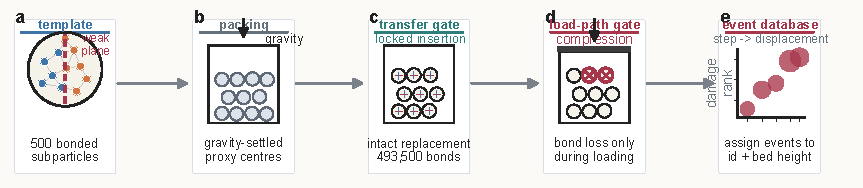
\includegraphics[width=0.92\textwidth]{../figures/main/fig1_workflow.pdf}
\caption{Locked-template workflow for fracture-resolved packed-bed compression. A nominal 1 mm bonded particle is represented by a 500-subparticle bonded template. Proxy spheres first settle under gravity without internal bonds. The settled proxy centres are replaced by intact bonded templates, so internal bond failure starts during compression. The entry-state record includes internal-bond conservation, native inter-particle force connectivity, six-wall force output and gravity-baseline-corrected incremental force balance. Bond-state records are then converted into a particle-resolved fracture-event database.}
\label{fig:workflow}
\end{figure}


\section{Methods}

\subsection{Bonded-particle template}

Each nominal 1 mm pebble is represented by 500 spherical subparticles connected by stress-breakable cohesive bonds. The selected weak-plane template uses bulk bonds away from a prescribed plane and weaker cross-plane bonds to reproduce a split-type failure mode. The template uses 4,935 initial internal bonds per parent particle. Single-pebble calibration runs use the same contact formulation as the bed calculations. The selected template is treated as a calibrated representation for event-sequence calculations within the tested sensitivity range.


\subsection{Locked-template bed construction}

Random beds are generated in two stages. First, 1 mm proxy spheres settle under gravity. Second, the final proxy centres are used as insertion sites for intact bonded templates generated in a separate dilute configuration. Atom-id ranges identify each parent particle after transfer. Selected 100-parent-particle beds contain 50,000 subparticles and 493,500 internal bonds before compression. The completed nominal and 0.25x-strength 200-parent-particle scale/strength endpoints each contain 100,000 subparticles and 987,000 internal bonds before compression.


\subsection{Entry-state loading}

Before fracture interpretation, each bed is checked for internal-bond conservation, measurable top-wall load transfer and a connected native force graph. Wall-force output is corrected by the gravity baseline from the settled state. The selected entry protocol uses five 1 micrometre step-relaxed increments, a restored contact modulus of $1.5\times10^{10}$ Pa and 10,000 pre-compression relaxation steps. The selected entry state retains all internal bonds and forms a top-to-bottom connected native force graph.


\subsection{Fracture-event extraction}

Compression runs write thermo histories, internal-bond local records and native pair/wall contact records. Broken-bond increments are obtained by comparing each internal-bond record with the intact reference graph. Broken bonds are assigned to parent-particle ids through atom-id ranges. The event table records displacement, parent-particle id, bond-loss increment, damaged-particle count and height rank. Native force-network descriptors are reconstructed from local contact forces between distinct parent particles.


\subsection{Strength matrix}

The repaired dataset adds a six-case strength matrix on two selected cracking geometries. Bulk and weak-plane normal/tangential bond strengths are scaled by 0.75, 0.50 and 0.25 relative to the nominal values. All six rows reach the 60 micrometre endpoint and are postprocessed into the same event and native-force-network tables as the nominal cases. The matrix records first localized bond-loss displacement, endpoint broken bonds, damaged parent-particle count, final inter-particle force sum, top reachability and bottom reachability from the top-loaded set.


The main template, contact, bond and loading parameters used across these calculations are summarized in Table 1.



\begin{table}[!t]
\centering
\caption{Model and bonded-template parameters}
\label{tab:model-parameters}
\scriptsize
\setlength{\tabcolsep}{2.2pt}
\renewcommand{\arraystretch}{1.12}
\begin{tabularx}{0.98\textwidth}{>{\raggedright\arraybackslash}p{0.29\textwidth}>{\raggedright\arraybackslash}p{0.18\textwidth}>{\raggedright\arraybackslash}X}
\toprule
Parameter & Value & Use in the calculations \\
\midrule
Parent-particle nominal diameter & 1.0 mm & Single-particle and bed calculations \\
Subparticles per parent particle & 500 & Bonded template \\
Initial internal bonds per parent particle & 4,935 & Intact template count before compression \\
Initial internal bonds per 100-parent-particle bed & 493,500 & Selected bed-window count before compression \\
Particle density & 2400 kg m$^{-3}$ & Contact dynamics and template mass \\
Young's modulus & 90 GPa & Hertzian contact input for single-particle calibration \\
Restored bed contact modulus & $1.5\times10^{10}$ Pa & Selected loaded-entry and bed compression protocol \\
Poisson ratio & 0.25 & Particle-particle and particle-wall contacts \\
Restitution coefficient & 0.3 & Normal damping in the contact law \\
Friction coefficient & 0.5 & Particle-particle and particle-wall contacts \\
Bond normal stiffness & $1.0\times10^{14}$ N m$^{-3}$ & Cohesive bonds \\
Bond tangential stiffness & $5.0\times10^{13}$ N m$^{-3}$ & Cohesive bonds \\
Bulk bond normal/tangential strength & 90 MPa & Bonds away from the weak plane \\
Weak-plane bond normal/tangential strength & 22.5 MPa & Reduced cross-plane bonds \\
Bulk bond-creation distance & 0.20 mm & Main internal bond network \\
Weak-plane bond-creation distance & 0.09 mm & Reduced cross-plane connectivity \\
Selected weak-plane orientation & x-normal & Reference template orientation \\
Single-particle loading velocities & 0.10, 0.05 and 0.03 m s$^{-1}$ & Loading-rate sensitivity \\
Bed displacement increment & 1 micrometre & Step-relaxed loaded-entry and compression runs \\
Bonded-template timestep & 5.0 ns & Single-particle and bonded-bed compression \\
Proxy-settling timestep & 1.0 microsecond & Unbonded proxy-sphere deposition \\
\bottomrule
\end{tabularx}
\end{table}


\section{Results}

\subsection{Single-particle template calibration}

The selected weak-plane template reaches the intended 1 mm crush-load scale and produces two dominant fragments with small chips (Fig. 2). The reference 500-subparticle case gives a peak top force of 18.64 N and a peak bottom force of 18.07 N. The final intact-bond graph contains two major fragments of 227 and 224 subparticles plus small chips. Orientation and strength-multiplier checks preserve the two-major-fragment mode while showing expected load scatter.


Resolution checks with 250, 500 and 1000 subparticles retain first-break displacement within 0.0950-0.0965 mm and preserve the two-fragment topology. Peak top force increases from 17.91 N at 250 subparticles to 19.40 N at 500 and 22.64 N at 1000, showing moderate residual load-scale sensitivity. Matched-boundary loading-rate checks at 0.10, 0.05 and 0.03 m s$^{-1}$ retain first-break displacement within 0.0945-0.0950 mm and preserve two dominant fragments. The 500-subparticle template is used for packed-bed event-sequence calculations with this sensitivity boundary.


\begin{figure}[!t]
\centering
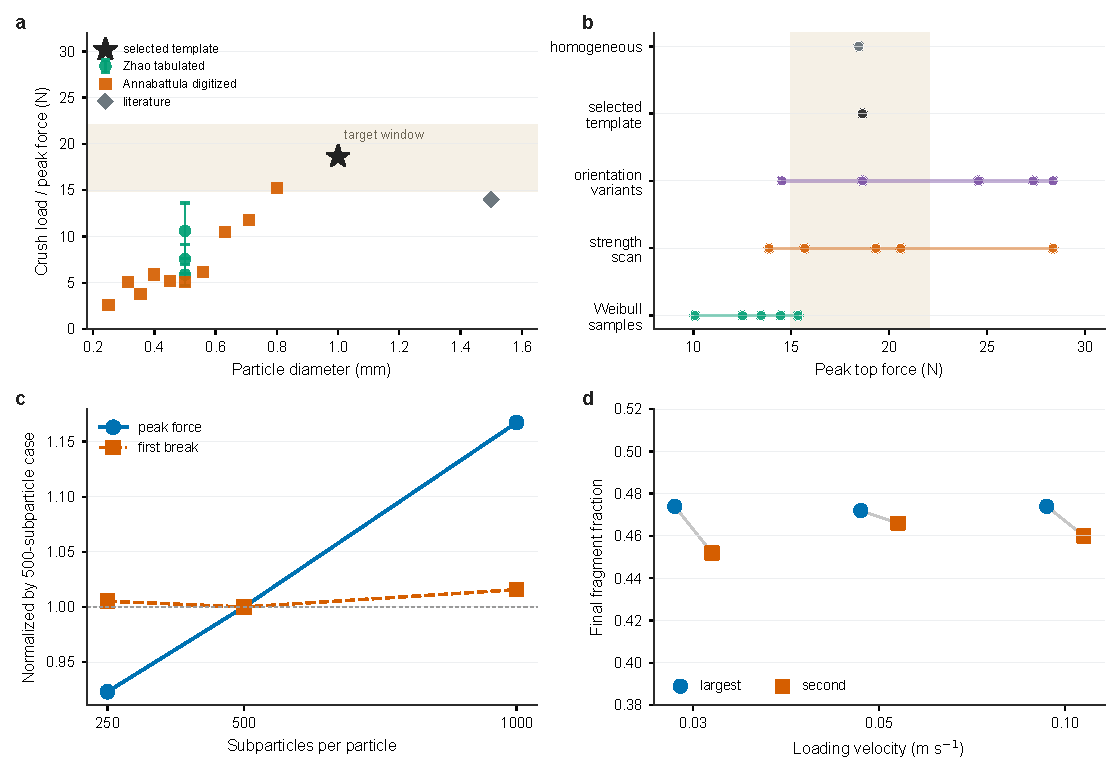
\includegraphics[width=0.92\textwidth]{../figures/apt_redesign/fig2_single_pebble_template_validation.pdf}
\caption{Single-pebble template selection and sensitivity. a, Published Li$_4$SiO$_4$ crush-load targets and the selected weak-plane bonded template. b, Peak-load distribution across homogeneous, selected weak-plane, orientation-variant, strength-scan and Weibull-sample calculations. c, Subparticle-resolution sensitivity, with peak force and first-break displacement normalized by the 500-subparticle template. d, Final largest- and second-largest-fragment fractions for matched-boundary loading-rate comparisons.}
\label{fig:single-pebble-template-validation}
\end{figure}


\subsection{Entry state before fracture loading}

The locked-template route creates selected 100-parent-particle beds with the expected 493,500 initial internal bonds. The selected entry protocol retains all internal bonds through five 1 micrometre increments (Fig. 3). At the selected 5 micrometre state, the final top-wall load is $1.638\times10^{-2}$ N and the gravity-baseline-corrected six-wall incremental force is $1.559\times10^{-2}$ N, giving a 4.799\% balance residual. The native force graph contains 36 inter-particle force edges and connects the top-loaded set to 28 parent particles, including three bottom-contacting particles.


The contact-modulus restoration series explains the chosen protocol. Zero pre-loading bond loss is retained at 5.0e8, 5.0e9 and 2.0e10 Pa, while 3.0e10 and 5.0e10 Pa introduce pre-loading bond loss. The $1.5\times10^{10}$ Pa entry state provides load transfer, a connected native force graph and intact internal bonds before fracture loading.


\begin{figure}[!t]
\centering
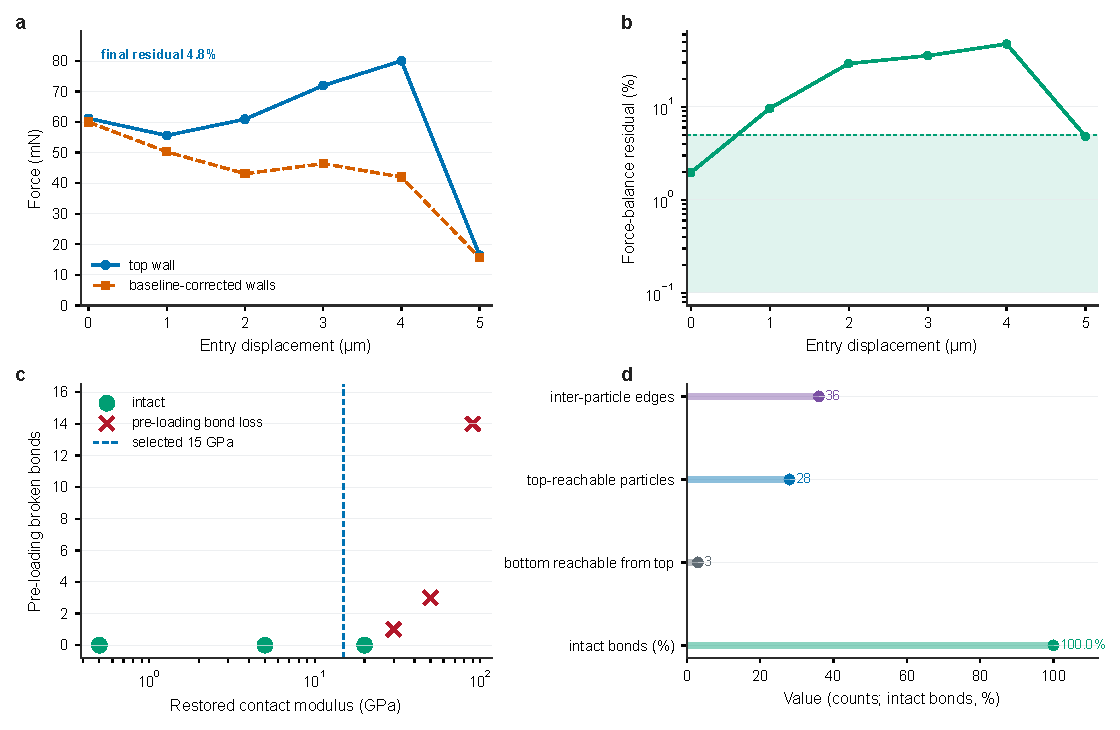
\includegraphics[width=0.92\textwidth]{../figures/apt_redesign/fig3_entry_state_validation.pdf}
\caption{Entry-state loading before fracture. a, Endpoint top-wall force and gravity-baseline-corrected wall force during the 5 micrometre entry protocol. b, Force-balance residual across entry displacement. c, Contact-modulus restoration series before fracture loading. d, Native final-state connectivity and intact-bond metrics for the selected entry state.}
\label{fig:entry-state-validation}
\end{figure}


\subsection{Fracture-event sequences}

The 60 micrometre compression runs resolve localized fracture-event sequences in finite 100-parent-particle windows (Fig. 4 and Table 2). The pilot sequence loses five of 493,500 internal bonds, all localized in one upper-bed parent particle. Event records contain three increments: two lost bonds at 25 micrometres, two additional lost bonds at 35 micrometres and one additional lost bond at 60 micrometres. The final native graph remains spanning, with 74 inter-particle force edges, 57 top-reachable parent particles and 11 bottom-contacting particles reachable from the top-loaded set.


An independent selected bed remains intact to 60 micrometres at nominal, 0.5x and 0.25x bond strengths. The final native graph remains spanning, with 83 inter-particle force edges, 67 top-reachable parent particles and 18 bottom-contacting particles reachable from the top-loaded set. Two 200-parent-particle scale/strength endpoints, at nominal and 0.25x strengths, also remain intact through 60 micrometres, each retaining all 987,000 internal bonds while ending with a spanning native graph, 53 inter-particle force edges, 43 top-reachable parent particles and eight bottom-contacting particles reachable from the top-loaded set. A delayed-cracking bed first loses bonds after 50 micrometres and ends with ten broken bonds localized in two upper-bed parent particles. Two additional selected cracking geometries provide early and synchronous fracture paths: the early-cracking geometry starts at 19 micrometres and the synchronous-cracking geometry starts at 39 micrometres under nominal strength. The current event table contains 11 localized event rows from four cracking cases.


\begin{figure}[!t]
\centering
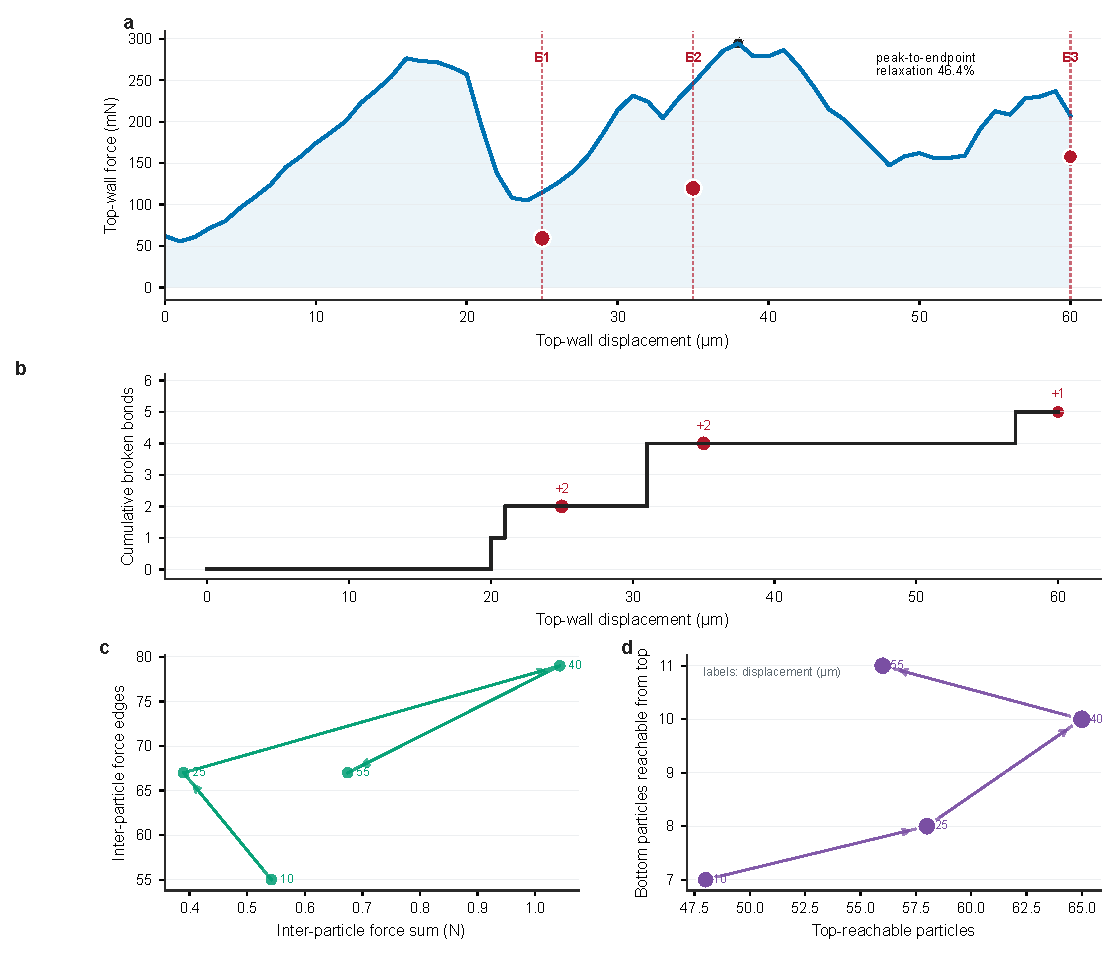
\includegraphics[width=0.92\textwidth]{../figures/apt_redesign/fig4_pilot_fracture_event_sequence.pdf}
\caption{Pilot fracture-event sequence and force-network evolution. a, Top-wall force envelope and particle-resolved event windows during the 60 micrometre pilot. b, Cumulative internal-bond loss from the thermo history with event localization. c, Native inter-particle force-network trajectory in force-sum versus edge-count space. d, Reachability trajectory for the top-loaded and bottom-reaching load path during the same sampled states.}
\label{fig:pilot-fracture-sequence}
\end{figure}



\begin{table}[!t]
\centering
\caption{Fracture-sequence results}
\label{tab:fracture-sequence}
\scriptsize
\setlength{\tabcolsep}{2.2pt}
\renewcommand{\arraystretch}{1.12}
\begin{tabularx}{0.98\textwidth}{>{\raggedright\arraybackslash}p{0.17\textwidth}>{\raggedright\arraybackslash}p{0.17\textwidth}>{\raggedright\arraybackslash}p{0.22\textwidth}>{\raggedright\arraybackslash}p{0.17\textwidth}>{\raggedright\arraybackslash}X}
\toprule
Quantity & Pilot bed & Intact bed and weakened-strength controls & Delayed-cracking bed & Interpretation \\
\midrule
Parent particles & 100 & 100 & 100 & Finite bed windows \\
Subparticles & 50,000 & 50,000 & 50,000 & 500 subparticles per parent particle \\
Initial internal bonds & 493,500 & 493,500 & 493,500 & Bonded templates transferred intact \\
Final intact internal bonds at 60 micrometres & 493,495 & 493,500 at nominal, 0.5x and 0.25x & 493,490 & Localized loss or zero loss at the endpoint \\
Damaged parent particles & 1 & 0 & 2 & Damage localizes in upper-bed parent particles \\
First thermo-resolved bond loss & 20 micrometres & none to 60 micrometres & 50 micrometres & Onset varies with local force path \\
Final inter-particle force edges & 74 & 83 & 63 & Native final force topology \\
Final top-reachable parent particles & 57 & 67 & 54 & Connected load-bearing graph \\
Final bottom-contacting particles reachable from top & 11 & 18 & 7 & Top-to-bottom force connectivity \\
\bottomrule
\end{tabularx}
\end{table}


\subsection{Mechanism variables}

The fracture sequences can be reduced to mechanism variables that are more informative than displacement history alone (Fig. 5 and Table 3). The cracking cases occupy higher inter-particle-force regions than the 100-parent-particle intact bed, weakened-strength controls and the two 200-parent-particle intact scale/strength checks. The pilot, delayed, early and synchronous cracking cases have final inter-particle force sums of 0.864, 1.032, 0.575 and 0.945 N, while the 100-parent-particle intact controls cluster near 0.253 N and the two 200-parent-particle intact endpoints both end near 0.113 N, all with zero internal-bond loss. Event-window topology shows both force-network densification and force-network reduction around localized bond-loss events.


The eleven-row material-response table gives a compact endpoint separation. Zero-loss endpoints have final inter-particle force sums of 0.113-0.253 N, whereas localized-cracking endpoints span 0.575-1.328 N. The smallest cracking value is 2.28 times the largest zero-loss value, and the midpoint between these ranges is 0.414 N for the current finite windows. Strength multiplier gives an overlapping coordinate: 0.25x, 0.50x and nominal strength all appear in both endpoint classes. Top-reachable counts also overlap between zero-loss and cracking cases. This pattern supports a joint state description built from force-path intensity, packing geometry, bond strength and event chronology.


The same endpoint contact networks were also mined for the upper tail of parent-particle contact forces. Localized-cracking cases have final 95th-percentile edge forces of 0.0382-0.0686 N, while zero-loss endpoints have 0.0119-0.0121 N. The finite-window F95 separation ratio is 3.16. The 99th-percentile edge force gives a second, stricter tail descriptor with a separation ratio of 1.86. These tail variables show that fracture onset is associated with the strongest native load-bearing contacts, not simply with the number of reachable particles in the load path.


The endpoint broken-bond fraction remains small, but the surrounding force network reorganizes measurably. In the pilot, the inter-particle edge count densifies by 1.44x before reorganization, the top-reachable population increases by 1.35x and the peak-to-endpoint top-wall force relaxes by 46.4\%. The event sequence, parent-particle identity, height rank, native reachability and force relaxation together describe local microcracking embedded in a connected load-bearing skeleton.


\begin{figure}[!t]
\centering
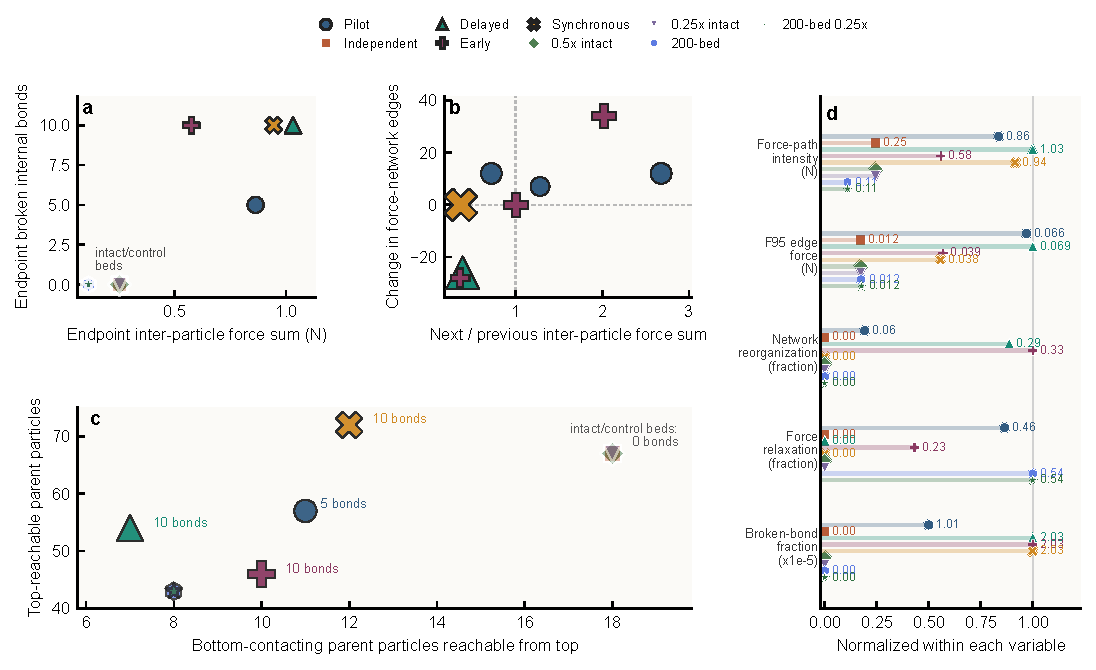
\includegraphics[width=0.98\textwidth]{../figures/pb007/pb007_replicate_comparison.pdf}
\caption{Mechanism variables for fracture onset. a, Endpoint mechanism map using summed inter-particle contact force and endpoint internal-bond loss. b, Event-window topology response for cracking cases, relating localized bond loss to the next-to-previous inter-particle force-sum ratio and the accompanying edge-count change. c, Native reachability map comparing bottom-contacting particles reachable from the top-loaded set with the total top-reachable parent-particle count. d, Normalized endpoint mechanism fingerprint, including total force-path intensity and the 95th-percentile edge force from the native parent-particle contact network. The endpoint table contains four cracking cases, three 100-parent-particle zero-loss controls and two 200-parent-particle zero-loss scale/strength endpoints; all retain spanning final native force graphs.}
\label{fig:mechanism-state-space}
\end{figure}



\begin{table}[!t]
\centering
\caption{Particulate breakage state-variable synthesis}
\label{tab:state-variables}
\scriptsize
\setlength{\tabcolsep}{2.2pt}
\renewcommand{\arraystretch}{1.12}
\begin{tabularx}{0.98\textwidth}{>{\raggedright\arraybackslash}p{0.20\textwidth}>{\raggedright\arraybackslash}p{0.30\textwidth}>{\raggedright\arraybackslash}p{0.25\textwidth}>{\raggedright\arraybackslash}X}
\toprule
State variable & Result in the present calculations & Physical interpretation & Scope \\
\midrule
Internal damage chronology & Four cracking cases provide 11 localized event rows & Converts hidden particle breakage into a time-ordered microcrack sequence & Four finite 100-parent-particle cracking windows \\
Damaged particle identity & The pilot damages one parent particle; delayed, early and synchronous paths damage two parent particles each & Identifies the local objects carrying early damage & One intact geometry remains unbroken to the endpoint \\
Native force-network state & Cracking cases retain spanning endpoint force graphs with 57-88 inter-particle force edges & Places local microcracking inside a connected load-bearing skeleton & Reconstructed from sampled native local contacts \\
Endpoint force-path separation & In 11 material-response endpoints, cracking rows have final inter-particle force sums of 0.575-1.328 N and zero-loss rows have 0.113-0.253 N & Identifies force-path intensity as a compact state coordinate & Separation ratio 2.28 in the current finite windows \\
Strong-force-tail separation & Cracking rows have final F95 edge forces of 0.0382-0.0686 N, while zero-loss rows have 0.0119-0.0121 N & Identifies the upper tail of native contact forces as the load-bearing region linked to fracture onset & F95 separation ratio 3.16; F99 separation ratio 1.86 \\
Macro-response accommodation & Endpoint forces span 0.158-0.649 N across cracking cases & Links microcracking to bed-window force evolution & Values are finite-window descriptors \\
Strength and scale response & The intact geometry remains unbroken at nominal, 0.5x and 0.25x; the 200-parent-particle bed remains unbroken at nominal and 0.25x through 60 micrometres; cracking geometries respond differently to strength reduction & Shows the combined role of local force path, scale window and material strength & Probability estimation requires larger ensembles \\
\bottomrule
\end{tabularx}
\end{table}


\subsection{Strength-dependent fracture response}

The completed strength matrix directly tests material-property dependence across two cracking geometries (Fig. 6 and Table 4). In the early-cracking geometry, first localized bond loss remains fixed at 19 micrometres from nominal strength through 0.25x strength. Endpoint bond loss stays at ten broken bonds for nominal, 0.75x and 0.50x strength, then increases to 15 broken bonds at 0.25x. Final inter-particle force sum increases from 0.575 N at nominal strength to 1.328 N at 0.75x, 1.196 N at 0.50x and 0.871 N at 0.25x.


The synchronous-cracking geometry shows a clearer onset shift. First localized bond loss moves from 39 micrometres at nominal strength to 29 micrometres at 0.75x and 19 micrometres at 0.50x and 0.25x. Endpoint bond loss stays at ten broken bonds for nominal, 0.75x and 0.50x strength, then increases to 15 broken bonds at 0.25x. Final inter-particle force sum is 0.945 N at nominal strength, 1.180 N at 0.75x, 0.853 N at 0.50x and 0.747 N at 0.25x. All six strength-matrix rows retain a spanning final native force graph.


\begin{figure}[!t]
\centering
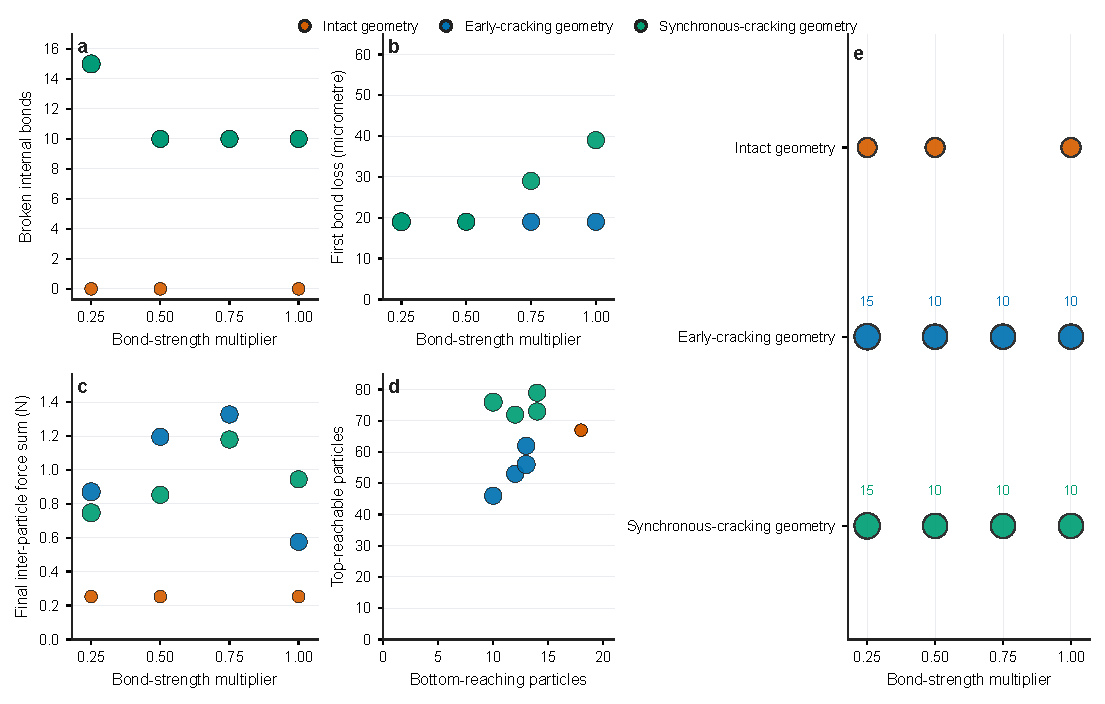
\includegraphics[width=0.92\textwidth]{../figures/pb007/pb007_material_strength_response.pdf}
\caption{Strength-dependent fracture response across cracking geometries. a, First localized bond-loss displacement as a function of bond-strength multiplier. b, Endpoint broken-bond count. c, Final inter-particle force sum. d, Native reachability descriptors at the endpoint. e, Matrix overview across intact, early-cracking and synchronous-cracking geometries. All plotted values are generated from the source table \texttt{data/figure\_source/pb007\_material\_strength\_response.csv}.}
\label{fig:material-strength-response}
\end{figure}



\begin{table}[!t]
\centering
\caption{Strength-matrix endpoint summary}
\label{tab:strength-matrix}
\tiny
\setlength{\tabcolsep}{2.2pt}
\renewcommand{\arraystretch}{1.12}
\begin{tabularx}{0.98\textwidth}{>{\raggedright\arraybackslash}p{0.18\textwidth}>{\centering\arraybackslash}p{0.10\textwidth}>{\centering\arraybackslash}p{0.14\textwidth}>{\centering\arraybackslash}p{0.12\textwidth}>{\centering\arraybackslash}p{0.12\textwidth}>{\centering\arraybackslash}p{0.12\textwidth}>{\centering\arraybackslash}X}
\toprule
Geometry class & Strength multiplier & First localized bond loss & Endpoint broken bonds & Damaged parent particles & Final force sum & Final top-reachable parents \\
\midrule
Early cracking & 1.00 & 19 micrometres & 10 & 2 & 0.575 N & 46 \\
Early cracking & 0.75 & 19 micrometres & 10 & 2 & 1.328 N & 53 \\
Early cracking & 0.50 & 19 micrometres & 10 & 2 & 1.196 N & 62 \\
Early cracking & 0.25 & 19 micrometres & 15 & 2 & 0.871 N & 56 \\
Synchronous cracking & 1.00 & 39 micrometres & 10 & 2 & 0.945 N & 72 \\
Synchronous cracking & 0.75 & 29 micrometres & 10 & 2 & 1.180 N & 79 \\
Synchronous cracking & 0.50 & 19 micrometres & 10 & 2 & 0.853 N & 73 \\
Synchronous cracking & 0.25 & 19 micrometres & 15 & 3 & 0.747 N & 76 \\
\bottomrule
\end{tabularx}
\end{table}


\section{Discussion}

The locked-template workflow resolves a practical difficulty in packed brittle-particle simulation: many internally bonded bodies can be placed into a load-bearing random bed while preserving their intact bond graphs. This makes the first few internal damage events measurable as a chronological dataset with direct parent-particle identity and native force-network state. The result complements bulk breakage-ratio and final-fragment measurements by exposing the particle-scale initiation history that occurs before bed-wide fragmentation.


The current calculations connect three scales. At the single-particle scale, the weak-plane template matches the available crush-load scale and split-type morphology within the tested resolution and rate sensitivities. At the initialization scale, the locked transfer creates selected 100-parent-particle beds with zero internal-bond loss and connected native force paths. At the fracture-sequence scale, the same records show localized microcracking embedded in spanning force graphs. The endpoint damage is small in absolute bond fraction, yet the surrounding force-network and macro-response descriptors change substantially.


The material-strength matrix adds direct material-property dependence to the event-sequence dataset. Strength reduction creates geometry-specific responses across random packings. One cracking geometry keeps the same first-event displacement as strength decreases and changes mainly in endpoint damage at 0.25x. The second cracking geometry advances its first event from 39 to 19 micrometres as strength decreases, then also increases endpoint damage at 0.25x. The intact geometry remains unbroken at nominal, 0.5x and 0.25x strength in the same displacement window. These finite-window results indicate that local force-path topology and bonded-particle strength jointly control early fracture.


The endpoint separation analysis gives the mechanism variables a quantitative role. Across 11 completed material-response endpoints, final inter-particle force sum separates the zero-loss and localized-cracking rows with a 2.28 force-intensity gap, while strength multiplier and top-reachable population overlap across endpoint classes. The force-tail descriptor adds a contact-level view of the same separation: cracking endpoints have an F95 edge-force range of 0.0382-0.0686 N, compared with 0.0119-0.0121 N for zero-loss endpoints. The result moves the interpretation from force-displacement reporting to a state-space description of early breakage. Local force intensity supplies the clearest endpoint coordinate in the present windows, the upper force tail identifies the contact subset that carries the fracture-prone load, and bond strength controls how each selected geometry moves through that state space.


The study remains bounded. The 100-parent-particle windows are designed for event-sequence resolution and mechanism-variable extraction, and the two 200-parent-particle intact endpoints provide nominal and 0.25x scale/strength comparisons within the same displacement window. Quantitative fracture probability, final Li$_4$SiO$_4$ material-law calibration and coupled thermal-flow prediction require larger random ensembles, slower cyclic histories and transport/contact-area coupling. The present dataset supplies the traceable intermediate layer: parent-particle damage chronology, local force-path state, scale-window comparison and material-strength response.


\section{Conclusions}

1. A 500-subparticle weak-plane bonded template provides a sensitivity-bounded 1 mm brittle-particle representation with split-type failure morphology.

2. Locked-template insertion creates selected 100-parent-particle beds with 493,500 initial internal bonds, zero pre-loading bond loss and connected native force paths before fracture loading.

3. The compression runs resolve parent-particle fracture-event sequences: four cracking cases produce 11 localized event rows, while three selected 100-parent-particle controls and two 200-parent-particle scale/strength endpoints remain intact to 60 micrometres.

4. Mechanism variables based on parent-particle identity, first-event displacement, endpoint bond loss, inter-particle force sum, strong-force-tail descriptors and native reachability expose fracture behavior that is hidden in bulk force-displacement histories; the final inter-particle force-sum gap between zero-loss and cracking endpoints is 2.28 and the F95 edge-force gap is 3.16 in the current material-response table.

5. The completed strength matrix shows geometry-specific material dependence: early-cracking onset remains fixed as strength decreases, whereas synchronous-cracking onset advances with strength reduction; both geometries increase endpoint bond loss at 0.25x strength.


\section{Data availability statement}

Processed event tables, native force-network summaries, material-response tables, figure source data and post-processing scripts are supplied as anonymous supplementary review files. Repository identifiers and author-linked archive information will be restored in the accepted version.


\section{Code availability statement}

Template-generation, run-control, figure-generation and post-processing scripts are supplied as anonymous supplementary review files. Author-linked repository identifiers will be restored in the accepted version.




\section{Declaration of competing interest}

The authors declare that they have no known competing financial interests or personal relationships that could have appeared to influence the work reported in this paper.



\bibliographystyle{elsarticle-num}
\bibliography{references}
\end{document}
